\documentclass[12pt]{article}
\usepackage{graphicx}
\usepackage{amsmath}

\begin{document}
CSCI-4100 Assignment 12 Yichuan Wang 661414395\\
1. Neural Network\\
(a)Back propagation:\\
Identity result:\\
Layer 1:\\
\[
\begin{bmatrix}
    -0.0322 & -0.0322 \\
    -0.0322 & -0.0322 \\
    -0.0322 & -0.0322
\end{bmatrix}
\]\\
Layer 2:\\
\[
\begin{bmatrix}
    -0.2162 &\\
    -0.1373 &\\
    -0.1373 &
\end{bmatrix}
\]\\\\
tanh result:\\
Layer 1:\\
\[
\begin{bmatrix}
    -0.0267 & -0.0267 \\
    -0.0267 & -0.0267 \\
    -0.0267 & -0.0267
\end{bmatrix}
\]\\
Layer 2:\\
\[
\begin{bmatrix}
    -0.1791 &\\
    -0.1137 &\\
    -0.1137 &
\end{bmatrix}
\]\\\\
(b) Gradient approximation with weight nudging by 0.0001\\
Identity result:\\
Layer 1:\\
\[
\begin{bmatrix}
    -0.0322 & -0.0322 \\
    -0.0322 & -0.0322 \\
    -0.0322 & -0.0322
\end{bmatrix}
\]
Layer 2:\\
\[
\begin{bmatrix}
    -0.2162 &\\
    -0.1373 &\\
    -0.1373 &
\end{bmatrix}
\]\\
tanh result:\\
Layer 1:\\
\[
\begin{bmatrix}
    -0.0267 & -0.0267 \\
    -0.0267 & -0.0267 \\
    -0.0267 & -0.0267
\end{bmatrix}
\]
Layer 2:\\
\[
\begin{bmatrix}
    -0.1790 &\\
    -0.1137 &\\
    -0.1137 &
\end{bmatrix}
\]\\
Conclusion: There is nearly no difference between forward propagation gradient estimation and back propagation method. \\\\
2. Neural Network with number digits\\
(a)\\
Error vs iteration:\\
Classifier: $E_{test}=0.0136$ \\
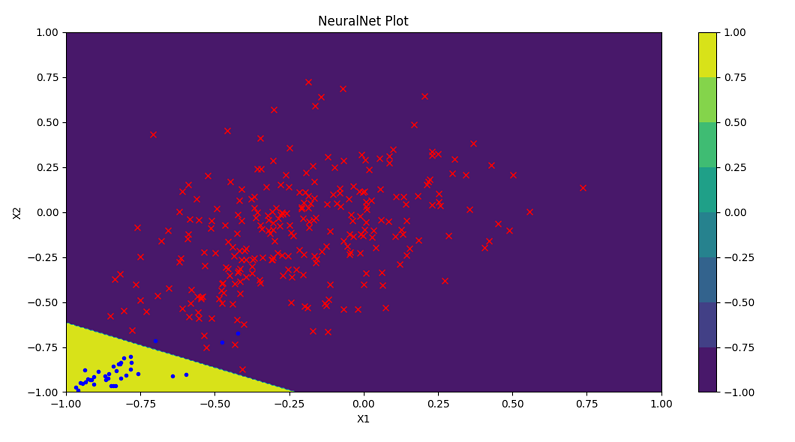
\includegraphics[scale=0.6]{images/nn1}\\\\
(b) Weight Decay with variable learning rate\\
Classifier: $E_{test}=0.0127$\\
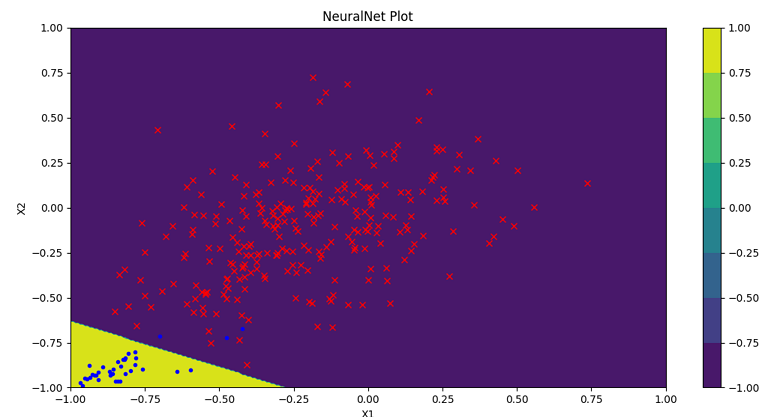
\includegraphics[scale=0.6]{images/nn2}\\\\
(c) Early stop\\
Classifier: $E_{test}=0.0126$\\
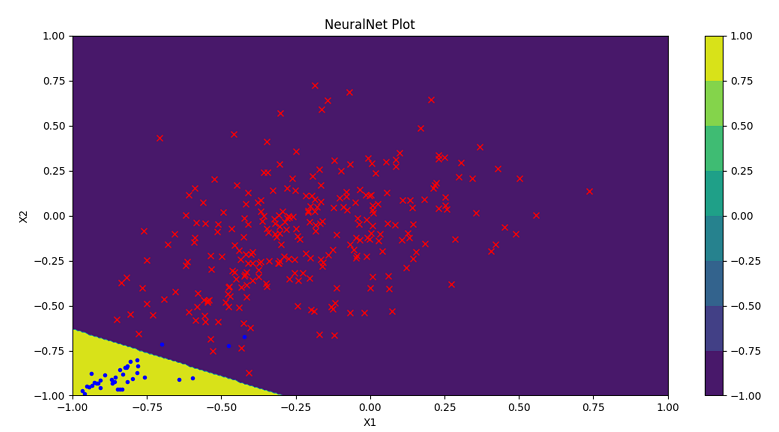
\includegraphics[scale=0.6]{images/nn3}\\\\\\
Since the data used last time is not saved, old models with new data (those used on NN) was run and data is provided below:\\
KNN: $E_{test} = 0.0174$\\
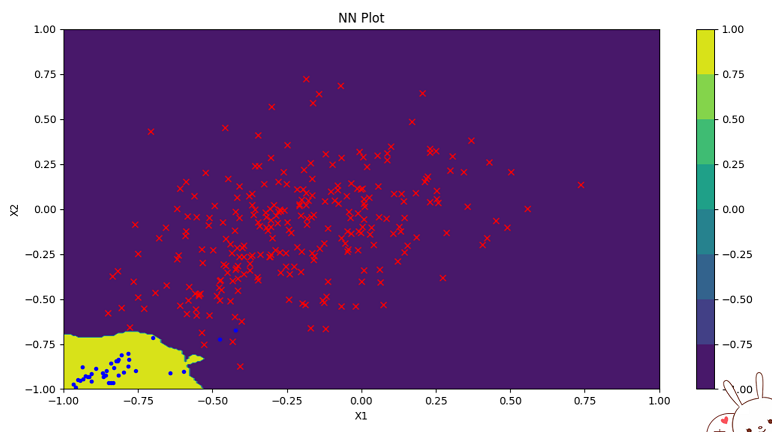
\includegraphics[scale=0.6]{images/nearest}\\
RBF: $E_{test} = 0.0144$\\
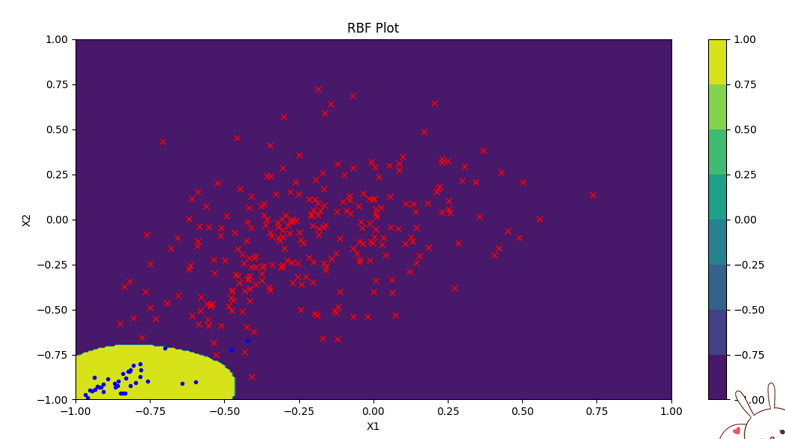
\includegraphics[scale=0.6]{images/rbf}\\
Linear Model: $E_{test} = 0.0284$\\
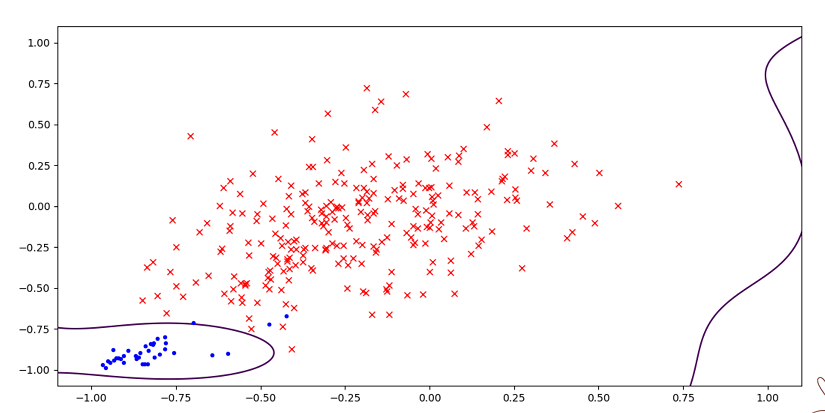
\includegraphics[scale=0.6]{images/linear_model}\\\\\\
3. SVM\\
(a) The optimal separator is $x_1=0$. Since two data points lay symmetrically about y axis, the y-axis gives the most cushion.\\
(b) After transformation, the data points lay symmetrically about the z1 axis, so $z_1=0$, the hyperplane
in the middle, gives the maximum cushion.\\
(c) After transformation the decision boundary becomes $z_1^3-z_2=0$, plot as following:\\
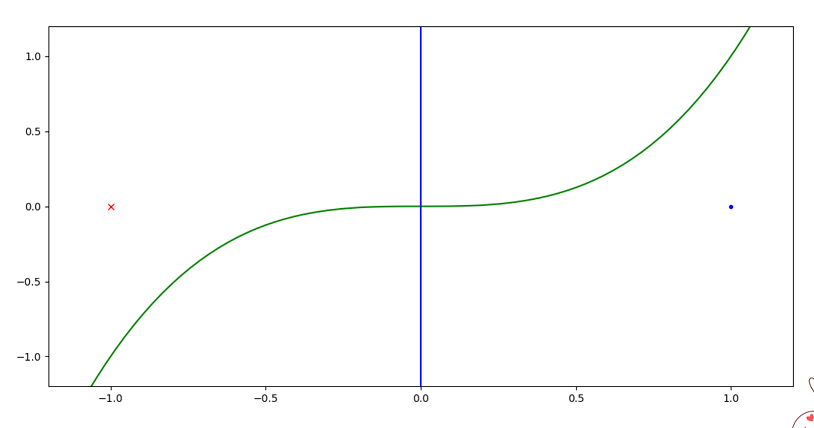
\includegraphics[scale=0.6]{images/svm_p3}\\
(d)\\
The data point after transformation is ($x_0^3-x_1, x_0x_1$), ($y_0^3-y_1, y_0y_1$)\\
Taking the dot product of these two we get following result:\\
$$x_0^3y_0^3-x_0^3y_1-y_0^3x_1+x_1y_1+x_0x_1y_0y_1$$\\
(e)The kernel function in function form is $h(x)=sign(x^3-y)$\\\\
4. SVM for digits\\
Small C is 0.1: $E_{test} = 0.0468$, image given below\\
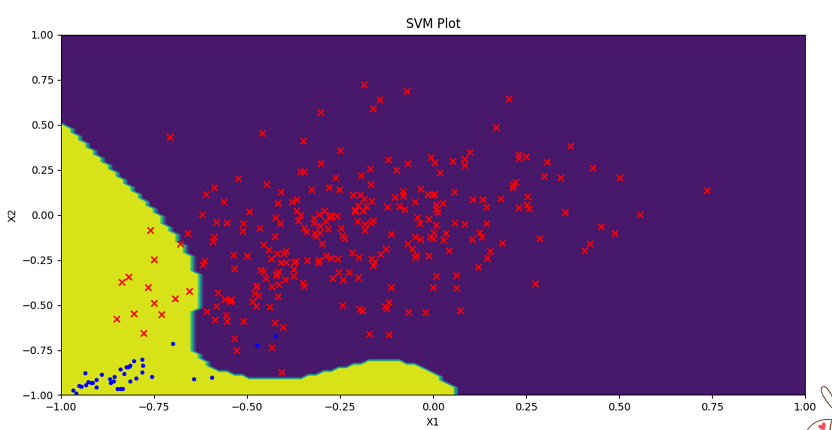
\includegraphics[scale=0.6]{images/svm_c01}\\
Large C is 100: $E_{test} = 0.0154$, image given below\\
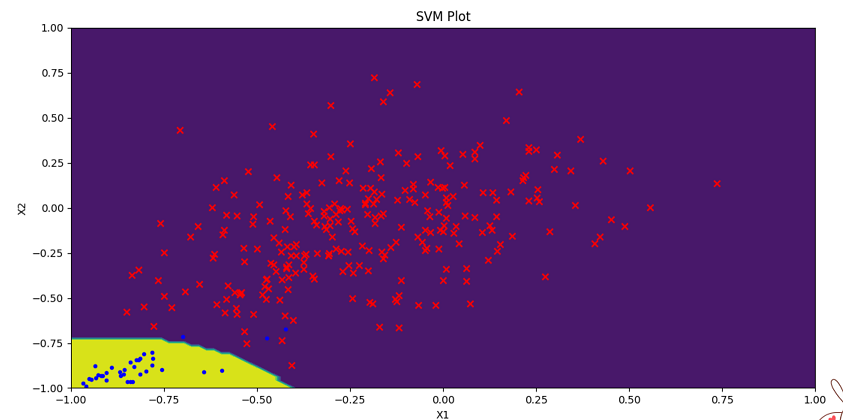
\includegraphics[scale=0.6]{images/svm_c100}\\
For cross validation choosing C from 0.1 to 100, $C=100$ has the best performance: ($E_{test}=0.0154$)\\
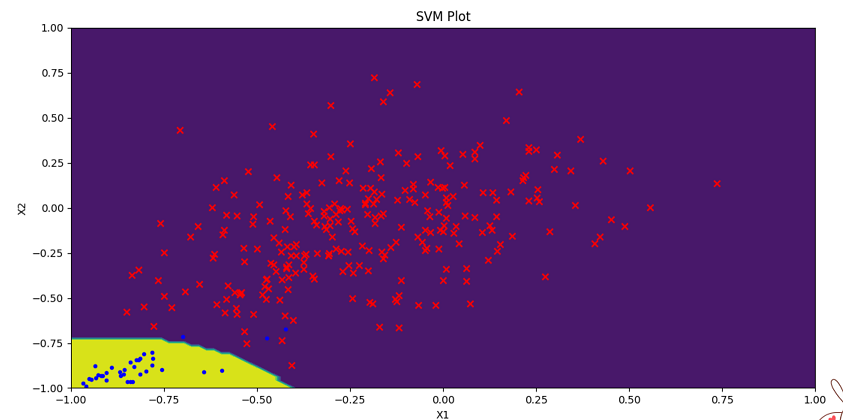
\includegraphics[scale=0.6]{images/svm_c100}\\
5. Comments\\
Test error comparison first:\\
Linear Model: 0.0284\\
KNN: 0.0174\\
RBF: 0.0144\\
Neural Network: 0.0126\\
SVM: 0.0154\\\\
Neural Network has the best result, and it's probably because it's high ability to fit the model, even though the final output classifier takes a linear fashion. SVM runs very fast, with an average performance; its ability to use cushion and use C to deal with inseparable data makes it more noise-resistant and that's probably why it's better than the linear model.\\
\end{document}












